%% LyX 2.0.4 created this file.  For more info, see http://www.lyx.org/.
%% Do not edit unless you really know what you are doing.
\documentclass[oneside,dutch]{amsart}
\usepackage[T1]{fontenc}
\usepackage[latin9]{inputenc}
\usepackage[a4paper]{geometry}
\geometry{verbose,tmargin=3cm,bmargin=3cm,lmargin=2cm,rmargin=2cm}
\setlength{\parskip}{\smallskipamount}
\setlength{\parindent}{0pt}
\usepackage{float}
\usepackage{amsthm}
\usepackage{graphicx}
\graphicspath{{Figures/}}

\makeatletter
%%%%%%%%%%%%%%%%%%%%%%%%%%%%%% Textclass specific LaTeX commands.
\numberwithin{equation}{section}
\numberwithin{figure}{section}

\makeatother

\usepackage{babel}
\begin{document}

\title{Spiegels}


\author{N.G. Schultheiss}

\maketitle

\section{Inleiding}

Deze module is direct te volgen vanaf de derde klas. Deze module wordt
vervolgd met de module ``Lenzen'' of de module ``Parabolische spiegels
maken''. Uiteindelijk kun je met de opgedane kennis een telescoop
bouwen, de werking verklaren of de telescoop als meetinstrument toepassen. 

Hieronder volgt een korte samenvatting van de kennis die je al beheerst.

De weerspiegeling van glanzende oppervlakken werkt met de spiegelwet.
Deze wet, ``De hoek van inval is de hoek van terugkaatsing'', voorspelt
hoe het licht wordt weerkaatst. 

\begin{figure}[H]
\noindent \begin{centering}
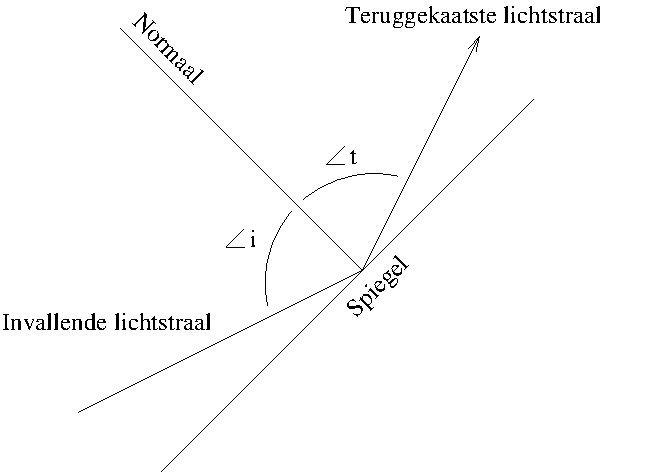
\includegraphics[scale=0.75]{spiegel}
\par\end{centering}

\caption{De stralengang van het licht bij een spiegel}
\end{figure}


In figuur 1 zie je hoe een gereflecteerde lichtstraal kan worden geconstrueerd.
De normaal staat altijd loodrecht op het spiegelend oppervlak. De
hoek van inval wordt altijd gemeten tussen de lichtstraal en de normaal.
De hoek van terugkaatsing wordt ook gemeten tussen de lichtstraal
en de normaal. We meten de hoek met de normaal, omdat we ook reflecties
van holle of bolle spiegels willen bepalen.

Omdat er getekend en gemeten moet worden, heb je een passer, geodriehoek,
potlood, papier en gum nodig.


\paragraph*{Opdracht 1:}

\emph{Meet de hoek van inval in figuur 1.} 


\section{Spiegeling aan bolvormige spiegels}

In een bolvormig oppervlak, zoals de achterkant van een lepel, zie
je de wereld verkleind. Aan de binnenkant van een lepel zie je de
wereld vergroot. Omdat een lepel niet precies bolvormig is, wordt
de wereld ook niet helemaal netjes afgebeeld. In deze paragraaf gaan
we uit van een bolvormige spiegel. De stralengang van het licht dat
van buiten op een glimmende bol valt kunnen we ook met de spiegelwet
voorspellen. Een dergelijk bol oppervlak heet ook wel ``convex''.

\begin{figure}[H]
\noindent \begin{centering}
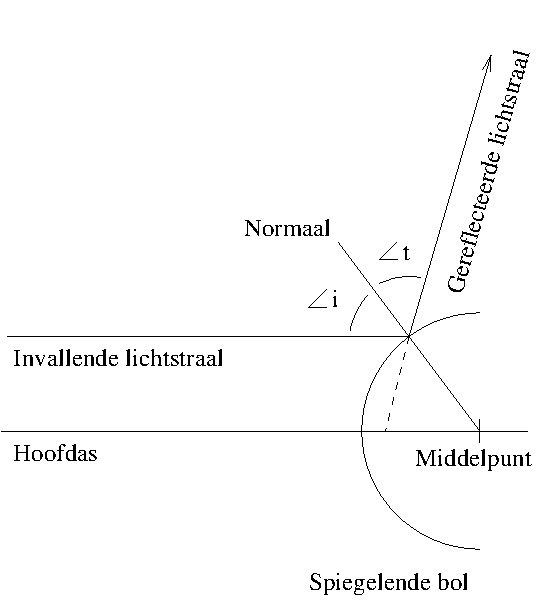
\includegraphics[scale=0.75]{bol}
\par\end{centering}

\caption{De stralengang bij een convex oppervlak}
\end{figure}


Als je in een spiegelende bol kijkt, zie je een beeld. Dit beeld wordt
een virtueel beeld genoemd.

Opdracht 1:

\emph{In figuur 2 zie je de normaal getekend. Leg uit waarom de normaal
door het middelpunt gaat.}

Opdracht 2:

\emph{Er valt een lichtbundel op je oog. Leg uit of je iets met een
convergente of een divergente bundel kunt zien.}

Opdracht 3:

\emph{Als een evenwijdige bundel op een bolle spiegel valt ontstaat
een gereflecteerde bundel. Wat voor soort bundel is deze gereflecteerde
bundel en leg uit of je deze kunt zien of niet.}

Een voor vergroting interessantere spiegeling is de stralengang bij
spiegeling aan de binnenkant van van een glimmende bol. Dit oppervlak
heet ook wel ``concaaf''. Hieronder zien we een lichtstraal die
in een hol oppervlak wordt gereflecteerd.

\begin{figure}[H]
\noindent \begin{centering}
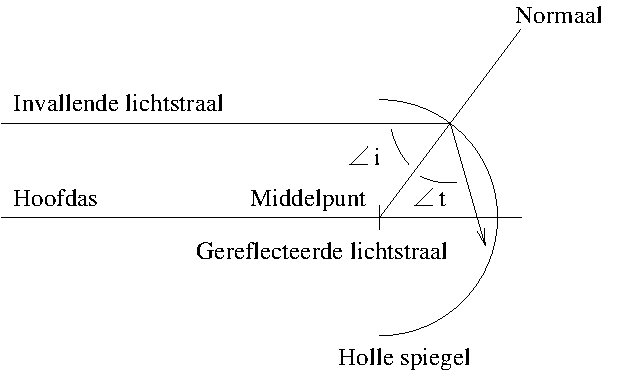
\includegraphics[scale=0.75]{hol}
\par\end{centering}

\caption{De stralengang bij een concaaf oppervlak}
\end{figure}


Een scherpe afbeelding is een afbeelding waarbij 1 punt van het voorwerp
als 1 punt van het beeld wordt afgebeeld. Er ontstaan lichtvlekjes
in het beeld als een afbeelding niet scherp is.

Opdracht 4:

\emph{Neem een stuk papier en teken daarop een holle spiegel met straal
van 5,0cm. Teken een evenwijdige bundel met vier stralen op 1,0cm,
2,0cm, 3,0cm en 4,0cm van de hoofdas. Construeer met de spiegelwet
hoe deze worden weerkaatst. Leg met je tekening / constructie uit
of een bolvormige spiegel te gebruiken is om scherpe afbeeldingen
te maken. }


\section{Parabolische en elliptische spiegels}

In paragraaf 2.3 hebben we gezien dat een bolvormige concave of convexe
spiegel geen keurig brandpunt oplevert. Bij een goede telescoop hebben
we een ander spiegelvorm nodig. In deze paragraaf proberen we te achterhalen
wat voor soort spiegelvorm het beste werkt.

We kunnen met het Huygens-principe voorspellen hoe het licht zich
als golf voortplant. Huygens beschreef het licht als golf. Een golf
kent twee eigenschappen; de golfstraal en het golffront. De golfstraal
is te vergelijken met de lichtstraal en geeft de richting aan waarin
de golf beweegt. Een golffront is bijvoorbeeld de ``top'' of het
''dal'' van de lichtgolf. Volgens het Huygens-principe is het volgende
golffront te vinden door op een golffront cirkeltjes met als straal
de golflengte te tekenen. Het volgende golffront is te schetsen door
een raaklijn (of rakende kromme) aan de cirkels te trekken.

\begin{figure}[H]
\noindent \begin{centering}
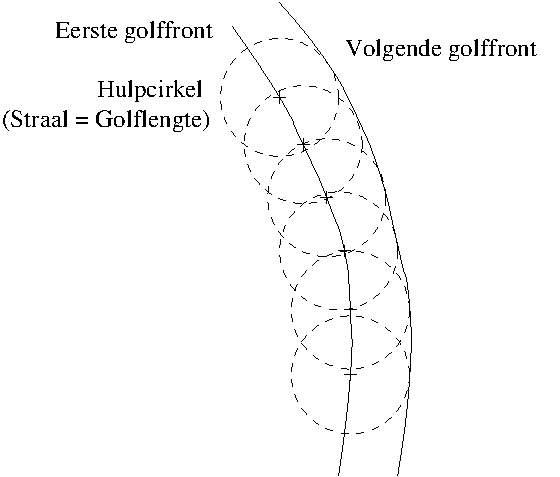
\includegraphics[scale=0.75]{huygens}
\par\end{centering}

\caption{Het Huygens-principe}
\end{figure}


Opdracht 1:

\emph{Leg uit dat het vorige golffront ook aan deze verzameling cirkeltjes
raakt.}

Opdracht 2:

\emph{Leg uit waarom een golffront altijd loodrecht op een golfstraal
staat.}

Een spiegel voor een telescoop moet een evenwijdige lichtbundel in
een punt afbeelden. Een evenwijdige lichtbundel is met het Huygens-principe
als een ruitjesblaadje voor te stellen. Als de horizontale lijntjes
de lichtstralen voorstellen, moeten de de verticale lijntjes de golffronten
voorstellen. Het licht gaat uiteindelijk naar 1 punt.

\begin{figure}[H]
\noindent \begin{centering}
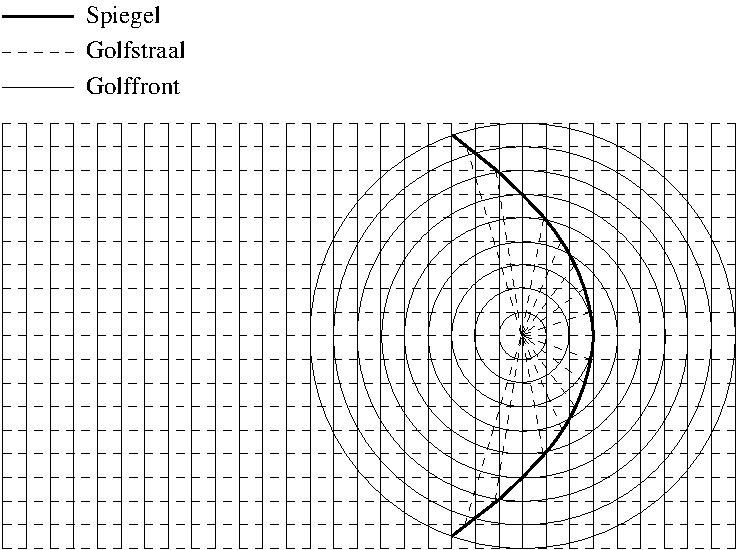
\includegraphics[scale=0.75]{parabool}
\par\end{centering}

\caption{Een Parabolische spiegel}
\end{figure}


Opdracht 3:

\emph{Leg met het Huygens-principe uit dat de golffronten cirkelvormig
worden als het licht }vanaf\emph{ of }naar\emph{ een punt gaat.}

Opdracht 4:

\emph{Leg uit dat je de vorm van de spiegel kunt vinden door de snijpunten
van de golffronten te verbinden. Wat gebeurd er met het golffront
bij de spiegel? Hoeveel golflengten legt het licht af om van links
tot aan het beeldpunt te komen? Is deze afgelegde weg verschillend
voor verschillende stralen?}

Opdracht 5:

\emph{Controleer of de spiegel parabolisch is.}

Met een spiegel kun je ook een afbeelding van een punt naar een punt
maken. In plaats van een evenwijdige invallende bundel hebben we nu
een divergente invallende bundel. Als deze divergente bundel uit 1
punt komt, zijn de golffronten weer als cirkels te tekenen.

Opdracht 6:

\emph{Teken een lichtpunt en een beeldpunt met de bijbehorende (mogelijke)
golffronten. Construeer een spiegel waarmee het lichtpunt op het beeldpunt
wordt afgebeeld. Deze spiegel wordt als het goed gaat een elips.}
\end{document}
